\chapter{Конструкторский раздел}

В данном разделе приведены ключевые алгоритмы использованные при написании драйвера сканера отпечатка пальца.

\section{Структура ПО}

Разрабатываемое ПО состоит из драйвера сканера отпечатка пальца и пользовательского приложения для тестирования работы драйвера.

\begin{figure}[h!]
    \centering
    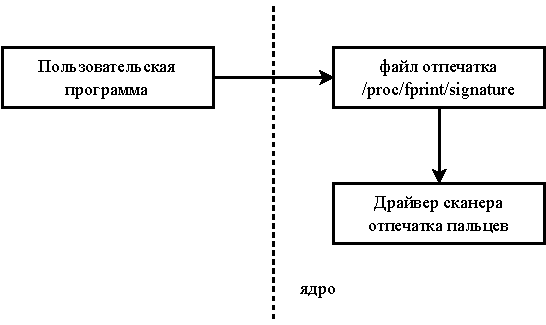
\includegraphics[width=0.9\textwidth]{img/structure-po}
    \caption{Структура ПО}
\end{figure}

\clearpage

\section{Алгоритм инициализации TLS-соединения}

На рисунке \ref{fig:init} представлен алгоритм инициализации TLS соединения с устройством. PSK \cite{psk} -- pre-shared key ciphersuites -- предварительный общий ключ безопасности используемый в качестве сертификата.

\begin{figure}[h!]
    \centering
    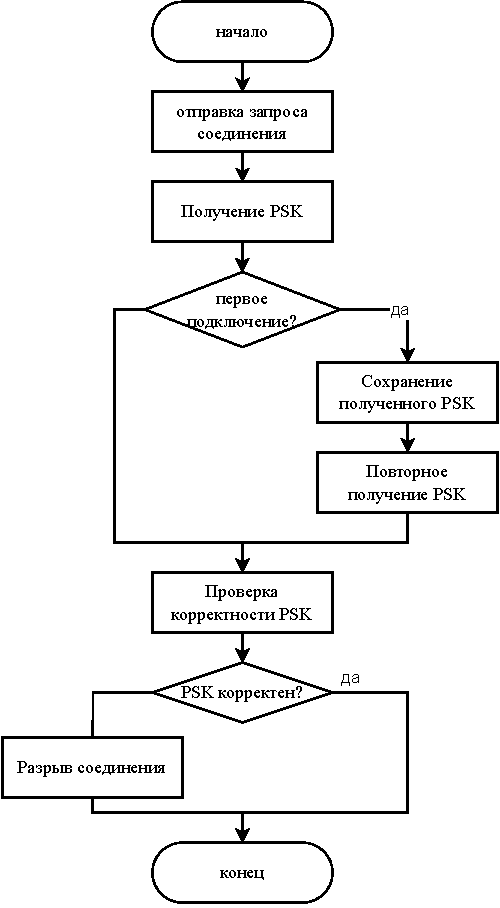
\includegraphics[width=0.6\textwidth]{img/init}
    \caption{Алгоритм инициализации соединения}
    \label{fig:init}
\end{figure}

\clearpage

\section{Обработка пользовательских запросов}

Сканер отпечатков пальцев является общим ресурсом для всех пользовательских приложений. Разрабатывая драйвер данного устройства важно рассмотреть все проблемы, которые могут возникнуть при обращении к драйверу различными пользовательскими приложениями в многопоточной системе.
Множество возможных проблем включает в себя следующие: 

\begin{enumerate}
    \item несколько пользовательских программ могут одновременно запрашивать отпечаток;
    \item несколько потоков одного процесса могут запрашивать отпечаток;
    \item процесс(поток) может умереть недочитав отпечаток;
    \item процесс(поток) может недочитать отпечаток.
\end{enumerate}

В качестве решения для указанных проблем можно предложить следующие подходы.

Во-первых, для обеспечения эффективной синхронизации захвата и использования ресурсов сканера отпечатков пальцев могут быть применены мьютексы, которые позволят ограничить доступ к общему ресурсу только одному потоку или процессу в определенный момент времени.

Кроме того, для решения проблемы прерванного чтения отпечатков пальцев можно ввести механизм отслеживания времени, чтобы по истечении определенного периода запрос отпечатка пальца был принудительно завершен. Это позволит избежать затянутого доступа к ресурсу в случае, если пользовательское приложение не успевает оперативно обработать данные от сканера.

Таким образом, разработка драйвера для сканера отпечатков пальцев в многопоточной системе требует учета и обработки указанных проблем с использованием вышеуказанных решений.

\clearpage

\section{Взаимодействие с ФС proc}

В контексте разработки драйвера сканера отпечатка пальцев важно иметь возможность передавать считанный отпечаток из пространства ядра в пространство пользователя. Для этого можно использовать интерфейс файлов последовательностей, предоставляемый ядром Linux. При этом данные считанного отпечатка будут представлены как последовательность байт, которую можно передать из пространства ядра в пространство пользователя с помощью файлов в виртуальной файловой системе \texttt{proc}. Диаграмма вызовов функций, определенных на \texttt{seq\_file} представлена на рисунке \ref{fig:seq-file}.

\begin{figure}[h!]
    \centering
    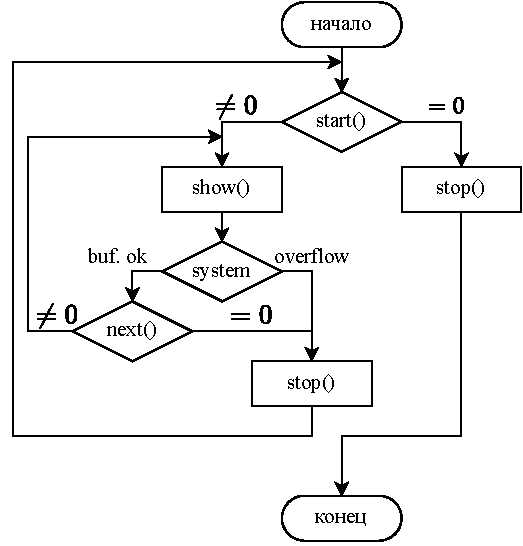
\includegraphics[width=0.7\linewidth]{img/seq-file.pdf}
    \caption{Диаграмма вызовов функций, определенных на \texttt{seq\_file}}
    \label{fig:seq-file}
\end{figure}

Альтернативными способами передачи отпечатка из пространства ядра в пространство пользователя могут быть использование специальных функций ядра, таких как \texttt{copy\_to\_user()} или системного вызова \texttt{mmap()}.

\clearpage

В случае разработки драйвера сканера отпечатка пальцев, использование интерфейса файлов последовательностей обосновано тем, что они предоставляют удобный механизм для передачи последовательности данных из ядра в пространство пользователя. Кроме того, они позволяют удобно осуществлять чтение и запись данных с использованием стандартных интерфейсов файловой системы, что упрощает взаимодействие пользовательских программ с драйвером сканера отпечатка пальцев.

\clearpage
